%%%%%%%%%%%%%%%%%%%%%
%   AMS packages    %
%%%%%%%%%%%%%%%%%%%%%
\documentclass[pdf]{beamer}
\usepackage{amsmath}
\usepackage{amsxtra}
\usepackage{amscd}
\usepackage{amsthm}
\usepackage{amsfonts}
\usepackage{amssymb}
\usepackage{eucal}
\usepackage[all]{xy}
\usepackage{graphicx}
\usepackage{comment}
\usepackage{amssymb}
\usepackage{latexsym,amsmath,amscd,amssymb,epsfig,verbatim}
%\usepackage{tikz}
%\usetikzlibrary{arrows,shapes}

\newtheorem{thm}{Theorem}
\newtheorem{cor}[thm]{Corollary}
\newtheorem{lem}[thm]{Lemma}
\newtheorem{prop}[thm]{Proposition}
\newtheorem{ex}[thm]{Exercise}
\newtheorem{conjecture}{Conjecture}
%\newtheorem*{conjecture*}{Conjecture}

\theoremstyle{remark}
\newtheorem{rem}[thm]{Remark}
\newtheorem{eg}[thm]{Example}

%\newtheorem{counterexample}[thm]{Counterexample}
\newtheorem{defn}[thm]{Definition}
%\newtheorem{claim}[thm]{Claim}
%\newtheorem{note}[thm]{Notation}
%\newtheorem{warning}[thm]{Warning}
%\newtheorem{variant}[thm]{Variant}
%\newtheorem{question}[thm]{Question}
%\newtheorem{construction}[thm]{Construction}
%\newtheorem{terminology}[thm]{Terminology}
%\newtheorem{convention}[thm]{Convention}

\newcommand\nc{\newcommand}
\nc\on{\operatorname}
\nc\renc{\renewcommand}
\newcommand\ssec{\subsection}
\newcommand\sssec{\subsubsection}
\newcommand\bO{{\mathbf O}}
\newcommand\CC{{\mathcal C}}
\newcommand\BN{{\mathbb N}}
\newcommand\BC{{\mathbb C}}
\newcommand\BF{{\mathbb F}}
\newcommand\BR{{\mathbb R}}
\newcommand\BQ{{\mathbb Q}}
\newcommand\BBZ{{\mathbb Z}}
\newcommand\uR{\underline{R}}
\newcommand\uZ{\underline{\BBZ}}
\newcommand\CF{{\mathcal F}}
\newcommand\uCF{\underline{{\mathcal F}}}
\newcommand\BZ{{\mathbb Z}}
\newcommand\BA{{\mathbb A}}
\newcommand\BP{{\mathbb P}}
\newcommand\fa{{\mathfrak a}}
\newcommand\fp{{\mathfrak p}}
\newcommand\fq{{\mathfrak q}}
\newcommand\fm{{\mathfrak m}}
\newcommand\pt{\mathrm{pt}}
\newcommand\rk{\operatorname{rk}}
\newcommand{\so}{\Rightarrow}
\newcommand{\upo}{\mathring}
\newcommand{\ra}{\rightarrow}
\renewcommand{\iff}{\Leftrightarrow}
\newcommand{\minus}{\backslash}
\renewcommand{\vec}[1]{\overrightarrow{#1}}
\renewcommand{\v}{\mathbf}
\newcommand{\gr}[1]{\langle {#1} \rangle}
\newcommand{\dstyle}{\displaystyle}
\newcommand\Aut{\operatorname{Aut}}
\nc{\bd}{\mathbf{d}}
\nc{\Hom}{\on{Hom}}
\nc{\End}{\on{End}}
\nc{\Spec}{\on{Spec}}
\nc{\Reg}{\on{Reg}}
\nc{\Specm}{\on{Specm}}
\nc\ol{\overline}
\nc\wt{\widetilde}
\nc{\one}{{\mathbf{1}}}
\renc{\mod}{\on{-mod}}
\newcommand{\id}{\mathrm{id}}
\nc{\ul}{\underline}
\nc{\uHom}{\ul\Hom}
\nc{\tHom}{\ul\uHom}
\nc{\wh}{\widehat}
\nc{\Vect}{\on{Vect}}
\nc{\Res}{\on{Res}}
\nc{\Ind}{\on{Ind}}



\newcommand\fbn{\mathcal H}
\newcommand \edgequot{\text{edge-quotient bijective }}

\def\Stab{\operatorname{Stab}}
\def\Fix{\operatorname{Fix}}
\newcommand\im{\text{Im}}


\AtBeginSection[]{
	\begin{frame}{Table of Contents}
		\tableofcontents[currentsection]
	\end{frame}
}

\mode<presentation>{}
\usetheme{Copenhagen}
\usecolortheme{seahorse}

%Title slide info goes here
\title{Peckness of Edge Posets}
\author{David Hemminger, Aaron Landesman, Zijian Yao}

\begin{document}

%Title Frame
\begin{frame}
	\titlepage
\end{frame}


\section{The Edge Poset and a Conjecture}

\begin{frame}{Definition of the Edge Poset}
\begin{defn}
\label{defn:functor_of_edges}
For $P$ a finite graded poset, it's \textit{edge poset} $\mathcal{E}(P)$ is the finite graded poset defined as follows. 
\begin{itemize}

\item Elements of $\mathcal{E}(P)$ are ordered pairs $(x,y)\in P\times P$ where $x\lessdot y$

\item Define $(x,y) \lessdot_{\mathcal{E}} (x^\prime,y^\prime)$ if $x\lessdot_P x^\prime$ and $y\lessdot_P y^\prime$

\item Define $\le_{\mathcal{E}}$ to be the transitive closure of $\lessdot_{\mathcal{E}}$

\item Define $\rk_{\mathcal{E}}(x,y) = \rk_P(x)$.
\end{itemize}
\end{defn}
\end{frame}

\begin{frame}
\begin{eg}
It is quite crucial we declare the relation $\leq_\mathcal F$ to be the transitive closure of $\lessdot_{\mathcal F}.$ An example of something that can go wrong is as follows. On the left hand side is the hasse diagram of a poset $P$ in the middle is the poset $\mathcal F^1(P)$ and on the right hand side is the poset obtained from the relation $x\otimes y \leq a\otimes b$ if $x \leq a, y \leq b.$

\[
\raisebox{1mm}{
\begin{tikzpicture}[scale=.7] at (0,0)
  \node (0) at (0,0) {$0$};
  \node (1) at (-1,2) {$1$};
  \node (2) at (1,2) {$2$};
  \node (3) at (0,4) {$3$};
  \node (4) at (2,4) {$4$};
  \node (5) at (0,6) {$5$};
  \node (6) at (2,6) {$6$};
  \node (7) at (1,8) {$7$};
  \draw (0)--(1);
  \draw (0)--(2);
  \draw (1)--(3);
  \draw (2)--(3);
  \draw (2)--(4);
  \draw (3)--(5);
  \draw (4)--(6);
  \draw (5)--(7);
  \draw (6)--(7);
  \node (8) at (0,-2) {$P$};
\end{tikzpicture}
}
\begin{tikzpicture}[scale = .7]
  \node (0) at (0,1) {$(0,1)$};
  \node (1) at (2,1) {$(0,2)$};
  \node (2) at (0,3) {$(1,3)$};
  \node (3) at (2,3) {$(2,3)$};
  \node (4) at (4,3) {$(2,4)$};
  \node (5) at (1,5) {$(3,5)$};
  \node (6) at (5,5) {$(4,6)$};
  \node (7) at (1,7) {$(5,7)$};
  \node (8) at (5,7) {$(6,7)$};
  \draw (0)--(2);
  \draw (1)--(3);
  \draw (1)--(4);
  \draw (2)--(5);
  \draw (3)--(5);
  \draw (4)--(6);
  \draw (5)--(7);
  \draw (6)--(8);
  \node (9) at (0,-2) {$\mathcal E^1(P)$};
\end{tikzpicture}
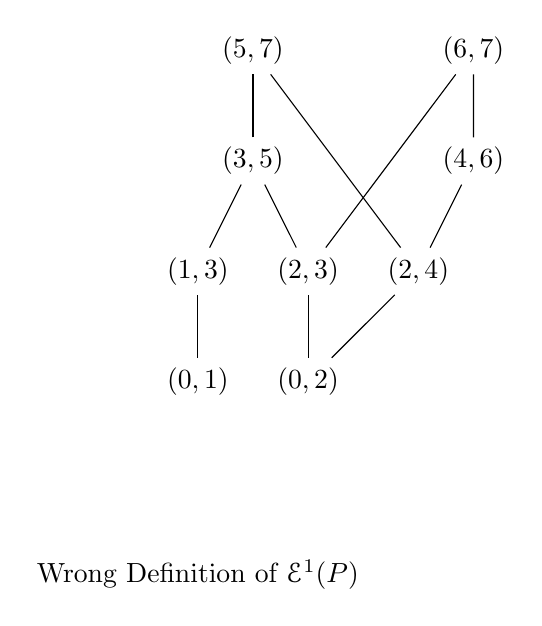
\begin{tikzpicture}[scale = .7]
  \node (0) at (0,1) {$(0,1)$};
  \node (1) at (2,1) {$(0,2)$};
  \node (2) at (0,3) {$(1,3)$};
  \node (3) at (2,3) {$(2,3)$};
  \node (4) at (4,3) {$(2,4)$};
  \node (5) at (1,5) {$(3,5)$};
  \node (6) at (5,5) {$(4,6)$};
  \node (7) at (1,7) {$(5,7)$};
  \node (8) at (5,7) {$(6,7)$};
  \draw (0)--(2);
  \draw (1)--(3);
  \draw (1)--(4);
  \draw (2)--(5);
  \draw (3)--(5);
  \draw (4)--(6);
  \draw (5)--(7);
  \draw (6)--(8);
  \draw (4)--(7);
  \draw (3)--(8);
  \node (9) at (0,-2.5) {$\text{Wrong Definition of } \mathcal E^1(P)$};
\end{tikzpicture}
\]
\fi

Here, it is clear that $\mathcal F^1(P)$ is a graded poset, with $rk(x\otimes y) = rk(x),$ but, the hasse diagram on the right represents a poset which does not have a grading.
\end{eg}

\end{frame}

\begin{frame}{A Conjecture on the Peckness of Edge Posets}
\begin{defn}
The \textit{boolean algebra of rank $n$} is the poset whose elements are subsets of $[n]$ with order given by containment, i.e. for $A,B\in B_n$, $A\le B$ if $A\subseteq B$.
\end{defn}


\begin{conjecture}[Hemminger, Landesman, and Yao 2014]
Let $G\subseteq \Aut(B_n)$.  Then $\mathcal{E}(B_n/G)$ is Peck.
\end{conjecture}
\end{frame}

\section{Main Result}
\subsection{Main Result}
\begin{frame}{Statement of Theorem}
\begin{defn}
A group action of $G$ on $P$ is \textit{cover transitive} if whenever $x,y,z\in P$ such that $x\lessdot z$, $y\lessdot z$, and $y\in Gx$, there exists some $g\in \Stab_G(z)$ such that $g\cdot x = y$.
\end{defn}

\begin{thm}[Hemminger, Landesman, and Yao 2014]
If a group action of $G$ on $B_n$ is cover transitive, then $\mathcal{E}(B_n/G)$ is Peck.
\end{thm}
\end{frame}

\subsection{Outline of Proof}

\begin{frame}
\begin{defn}
Given a group action of $G$ on $P$, we define a group action of $G$ on $\mathcal{E}(P)$ by letting $g\cdot (x,y) = (g\cdot x,g\cdot y)$ for all $g\in G$.
\end{defn}
\pause
\begin{prop}
The map $q\colon \mathcal{E}(P)/G\rightarrow \mathcal{E}(P/G)$ defined by $q(G(x,y)) = (Gx,Gy)$ is a surjective morphism.  Furthermore, $q$ is also injective if and only if the action of $G$ on $P$ is cover transitive.
\end{prop}

\begin{lem}
If $f:P\rightarrow Q$ is a bijective morphism and $P$ is Peck then $Q$ is Peck.
\end{lem}
\end{frame}

\begin{frame}
It then suffices to show that $\mathcal{E}(P)/G$ is Peck.  The following theorem will be useful.

\begin{thm}[Stanley, 1984]
If $P$ is unitary Peck and $G\subseteq\operatorname{Aut}(P)$, then $P/G$ is Peck.
\end{thm}
\end{frame}




\end{document}